    \documentclass{article}

    \usepackage{hyperref}
    \usepackage{graphicx}
    \usepackage{float}



    \hypersetup{
        colorlinks=true,
        linkcolor=blue,
        filecolor=magenta,
        urlcolor=cyan,
    }

    \author{Kolobok team}
    \title{OCR Research results}
    \date{June 2025}

\begin{document}
\maketitle

\section{Introduction}

During this week sprint, we were mainly focused on the OCR pipeline (recognizing tire mark, manufacturer, and size). Below is the summary of our work.

\section{Research}

Our investigation of existing solutions yielded the following sources:

\begin{itemize}
    \item \href{https://www.griddynamics.com/blog/how-to-identify-vehicle-tires-using-deep-learning-visual-models}{Grid Dynamics} - a blog post about the implementation of an application with similar to our functionality. Their pipeline consists of detection of the tire ring, then unwrapping it and applying OCR.
    \item \href{https://blog.roboflow.com/best-ocr-models-text-recognition/}{Roboflow} - a blog post with a comparison results of different OCR models on different datasets, including tire marks. \ref{fig:comp_table} shows their results.
    \item \href{https://github.com/open-mmlab/mmocr}{MMOCR} - an open-source library by OpenMMLab, which contains a collection of modern OCR pipelines, including text detection and recognition.
    \item \href{https://github.com/tesseract-ocr/tesseract}{Tesseract} - an open-source end-to-end OCR engine by Google.
\end{itemize}

\begin{figure}[H]
    \centering
    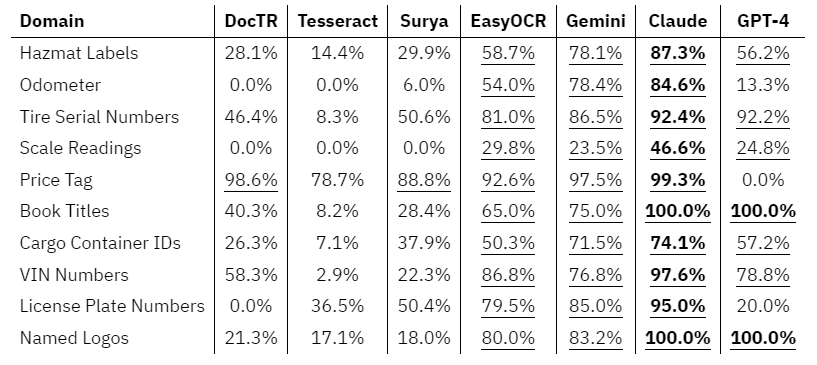
\includegraphics[width=0.8\textwidth]{assets/comp_table.png}
    \caption{Comparison of different OCR models on different datasets, including tire marks by Roboflow blog post}
    \label{fig:comp_table}
\end{figure}

\section{Experiments}

In order to evaluate existing approaches, we collected a small dataset of 15 images with side view of tires from parking near the 6th dormitory. Then we evaluated the accuracy of different models and different image preprocessing approaches. Our conducted experiments include the following DL pipelines:

\begin{itemize}
    \item \textbf{Tesseract}
    \item \textbf{DBNet++} + \textbf{ABINet} (MMOCR)
    \item \textbf{PSENet} + \textbf{ABINet} (MMOCR)
    \item \textbf{TextSnake} + \textbf{ABINet} (MMOCR)
    \item \textbf{PANet} + \textbf{ABINet} (MMOCR)
    \item \textbf{GPT-4o-mini}
\end{itemize}

In MMOCR models, we use a combination of two models: text detector (first) and text recognition (second). We evaluated the pipeline with varying text detection models, while preserving the same recognition model. We argue that our pipeline quality is more dependent on the detection model (for example, TextSnake is better at detecting curved text, while DBNet++ is better at finding bounding boxes of text), while recognition models from MMOCR model zoo show similar performance on same datasets. Therefore, to get an accurate comparison results, we keep the recognition model constant for all experiments (Note: ABINet is the latest model in MMOCR repository).

We also evaluated proposed algorithms on different preprocessing approaches:

\begin{itemize}
    \item \textbf{Raw} - no preprocessing
    \item \textbf{Polar unwrapping} - unwrapping the tire image to a flat view (see \ref{fig:unwrapped_tire})
    \item \textbf{CLAHE} - contrast limited adaptive histogram equalization (see \ref{fig:clahe_example})
\end{itemize}

\begin{figure}[H]
    \centering
    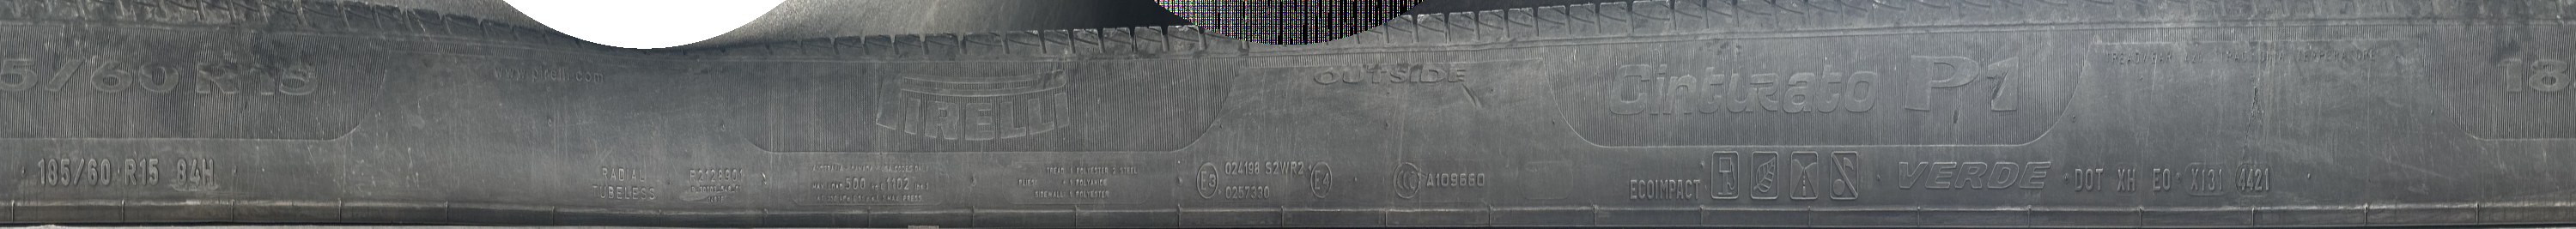
\includegraphics[width=1.\textwidth]{assets/unwrapped_example.png}
    \caption{Unwrapped tire image example}
    \label{fig:unwrapped_tire}
\end{figure}

\begin{figure}[H]
    \centering
    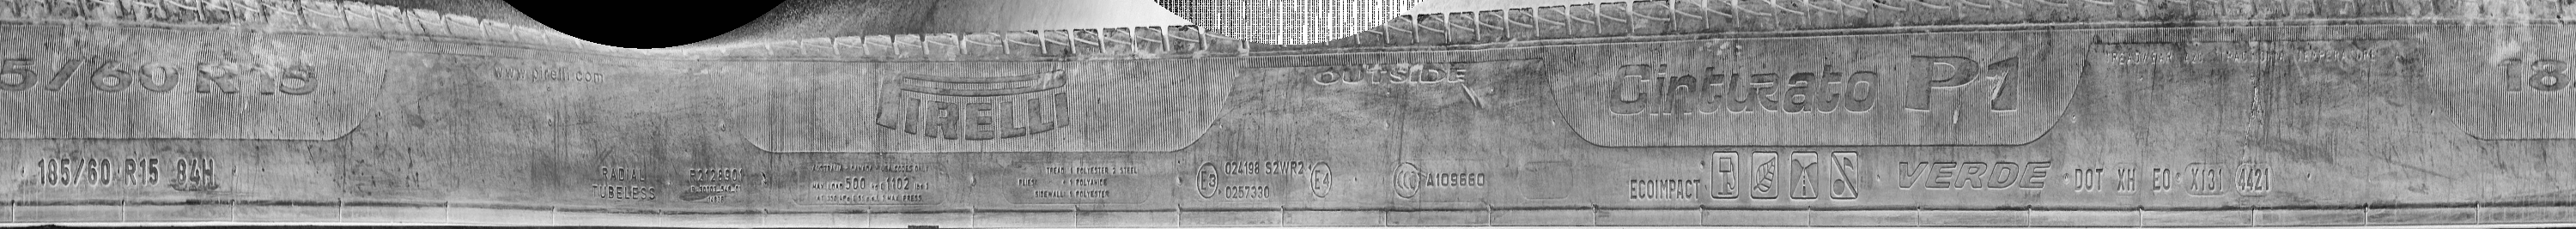
\includegraphics[width=1.\textwidth]{assets/clahe_example.png}
    \caption{CLAHE-enhanced tire image example}
    \label{fig:clahe_example}
\end{figure}

\section{Evaluation details}

We conduct an evaluation session, where the image is first preprocessed, then passed through the OCR pipeline, and finally the output is compared with the ground truth.

Evaluation metric: the number of correctly recognized texts. We have 3 labels for each image: tire mark, manufacturer, and size, giving 45 text labels in total. For each pipeline, we evaluate the number of correctly recognized texts.

For Tesseract and MMOCR models, we do not use any postprocessing of output, which gives an advantage to GPT-4o-mini, which can apply its knowledge of the language to get more accurate results. To compensate for this bias, we evaluate those models in the following way:

\begin{itemize}
    \item All of the detected texts are compared with all GT labels
    \item If the detected text has a levenstein ratio with any GT label more than 0.75, it is considered as correctly recognized
\end{itemize}

This approach gives more tolerance to the OCR models without language knowledge, as spelling mistakes can easily be corrected later.

GPT-4o-mini is evaluated more strictly:
\begin{itemize}
    \item The model is instructed to output \texttt{JSON} data with 3 fields
    \item Each field is compared with GT label, and considered correct only if there is a perfect match
\end{itemize}

\section{Results}

\begin{table}[H]
    \centering
    \begin{tabular}{|l|c|c|c|}
        \hline
        \textbf{Model}     & \textbf{Raw} & \textbf{Polar Unwrapping} & \textbf{CLAHE} \\
        \hline
        Tesseract          & 4            & 9                         & 8              \\
        \hline
        DBNet++ + ABINet   & 6            & 10                        & 15             \\
        \hline
        PSENet + ABINet    & 5            & 11                        & 14             \\
        \hline
        TextSnake + ABINet & 7            & 12                        & 16             \\
        \hline
        PANet + ABINet     & 3            & 8                         & 9              \\
        \hline
        GPT-4o-mini        & 37           & 45                        & 45             \\
        \hline
    \end{tabular}
\end{table}

\section{Conclusion}

As our experiments have shown, the most accurate approach is to use GPT-4o-mini with unwrapping preprocessing with optional CLAHE. We may consider using an approach less dependent on external APIs, but it would require proper tuning of the OCR pipelines, which is not a strict requirement, as GPT-4o-mini API cost is very low.

\end{document}